\documentclass[10pt]{article}
\usepackage[letterpaper]{geometry}
\usepackage{listings}
\usepackage{graphicx}
\renewcommand{\figurename}{Imagen}


\title{\textbf{Reporte: Interbloqueos}}
\author{Diego Ruiz Mora | 2202000335}
\date{9-Octubre-2023}

\begin{document}
	
	\maketitle
	\section{Variables Globales}
	Todos los programas contienen un par de variables globales con el mismo propósito en todos los programas.  Notaremos que solo el ultimo de los códigos  usará la variable global que esta comentada, que funcionará para hacer el conteo de veces que se ejecutan los hilos. 
	\begin{figure}[h!]
		\centering
		
\includegraphics[width=\linewidth]{valGob.png}
		\caption{Variables Globales}
		\label{fig:vg}
	\end{figure}
	Encontraremos la variable \emph{almacén} del tipo arreglo de caracteres con una longitud de diez, que servirá para mostrar los productos generados o consumidos. Por otro lado tenemos \emph{condc} y \emph{condp} que son variables de condición que nos permite bloquear los hilos si cumplen ciertas condiciones o igual despertar estos hilos en caso de cumplir ciertas características.  A su vez, tenemos también una variable del tipo mutex \emph{candado}  que nos ayudará a delimitar la región crítica y el acceso de cada uno de los hilos a la misma. Por último las variables enteras de \emph{pos} que indica la posición dentro del almacén y el contador, que ya se mencionó su uso.  
	\section{Funciones del programa}
	Muchas de las funciones de los códigos son iguales, algunas solo varían en una pequeña cosa, de manera conveniente explicaremos la función solamente una vez para ahorrarnos la necesidad de repetirlo en cada uno de los códigos.  
	\subsection{Función Principal}
	Comenzamos por la función principal, donde encontramos la declaración de variables del tipo \textbf{pthread\_t} que serán los dos hilos que utilizamos para consumir y producir elementos dentro del almacén. Para ello tenemos que inicializar las variables de condición para cada uno de los hilos, además hacemos la creación de los hilos dándoles como imagen la función \emph{intentaRegionCritica}, recordemos que tenemos que esperar a que termine de ejecutar cada uno de los hilos creados. 
	\\\\
	Para finalizar destruimos las condiciones y el candado, esto con las ultimas tres instrucciones. donde pasamos por referencia los valores de los respectivos.  
	\begin{figure}[h!]
		\centering
		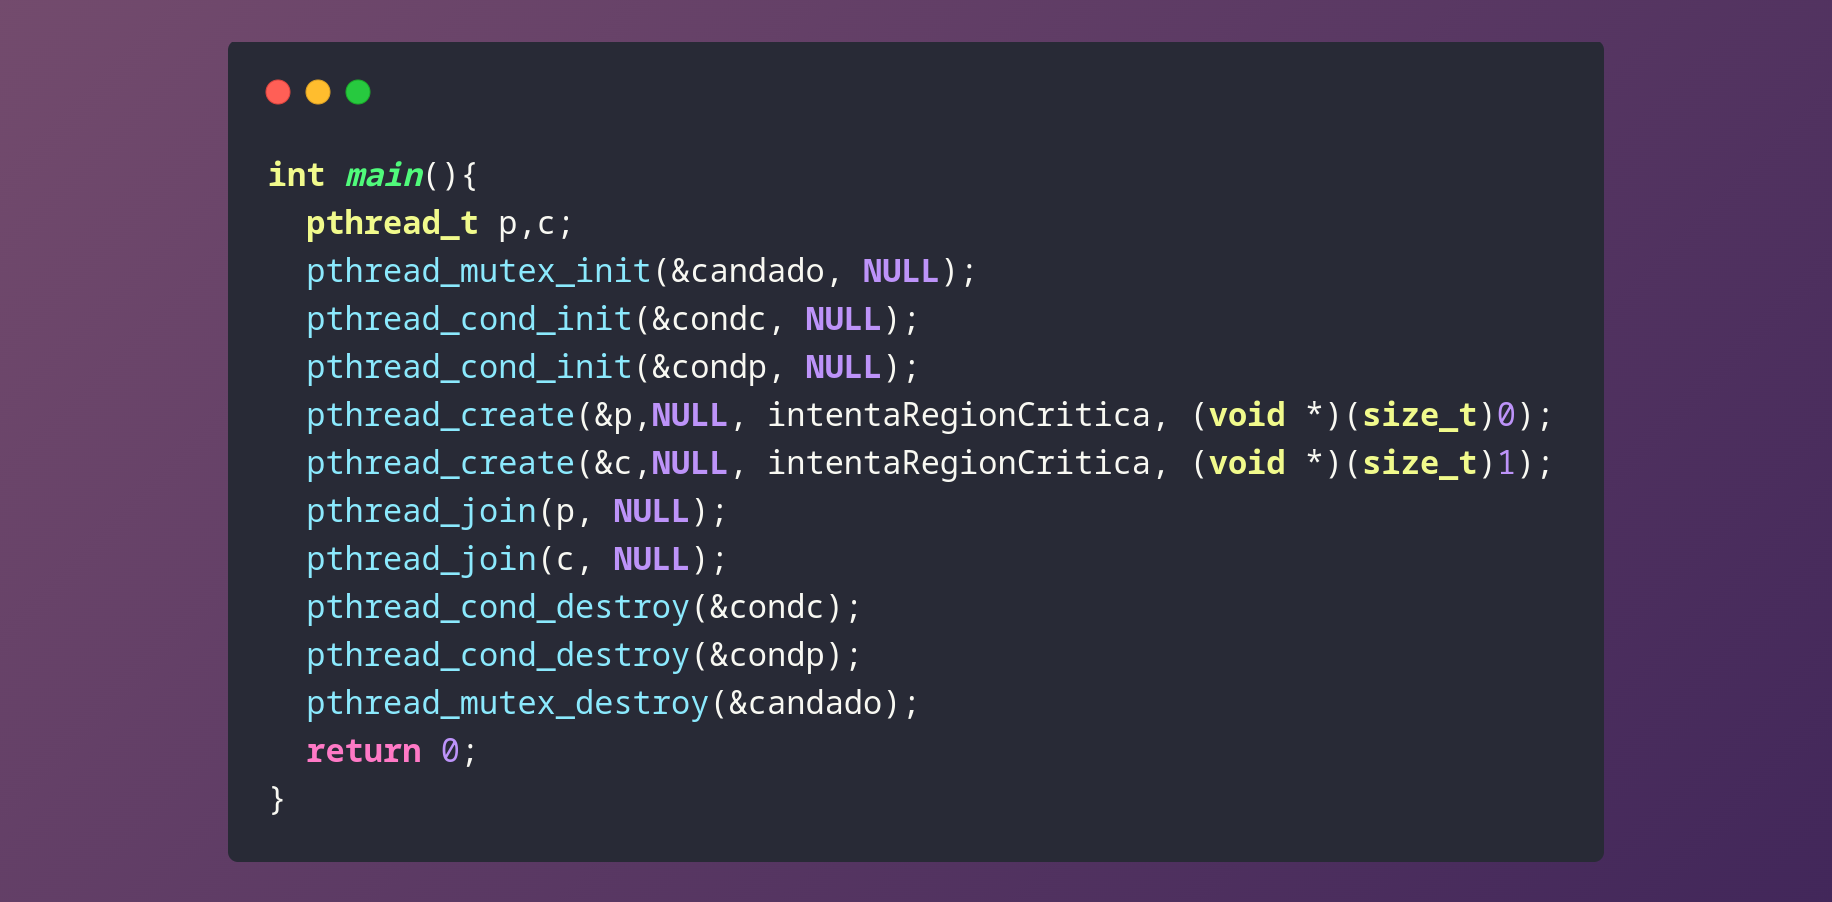
\includegraphics[width=\linewidth]{main.png}
		\caption{Función Principal}
		\label{fig:main}
	\end{figure}
	\subsection{Función para cada hilo}
	La llamada función \emph{intentaRegionCritica} que es la imagen de cada uno de los hilos recibe como parámetro el número de hilo, que justamente nos funcionará para identificar que función particular ejecutará, si la de consumir o la de producir, pero para ello primero tenemos que generar un ciclo de cincuenta repeticiones y dentro de el haremos la delimitación de la región critica para que cada uno de los hilos puedan acceder de manera ordenada  a ella. La delimitación laharemos abriendo y cerrando el mutex, todo esto dentro del ciclo, para que lo repita cincuenta veces por cada uno de los hilos, para darnos un total de cien veces. 
	\begin{figure}[h!]
		\centering
		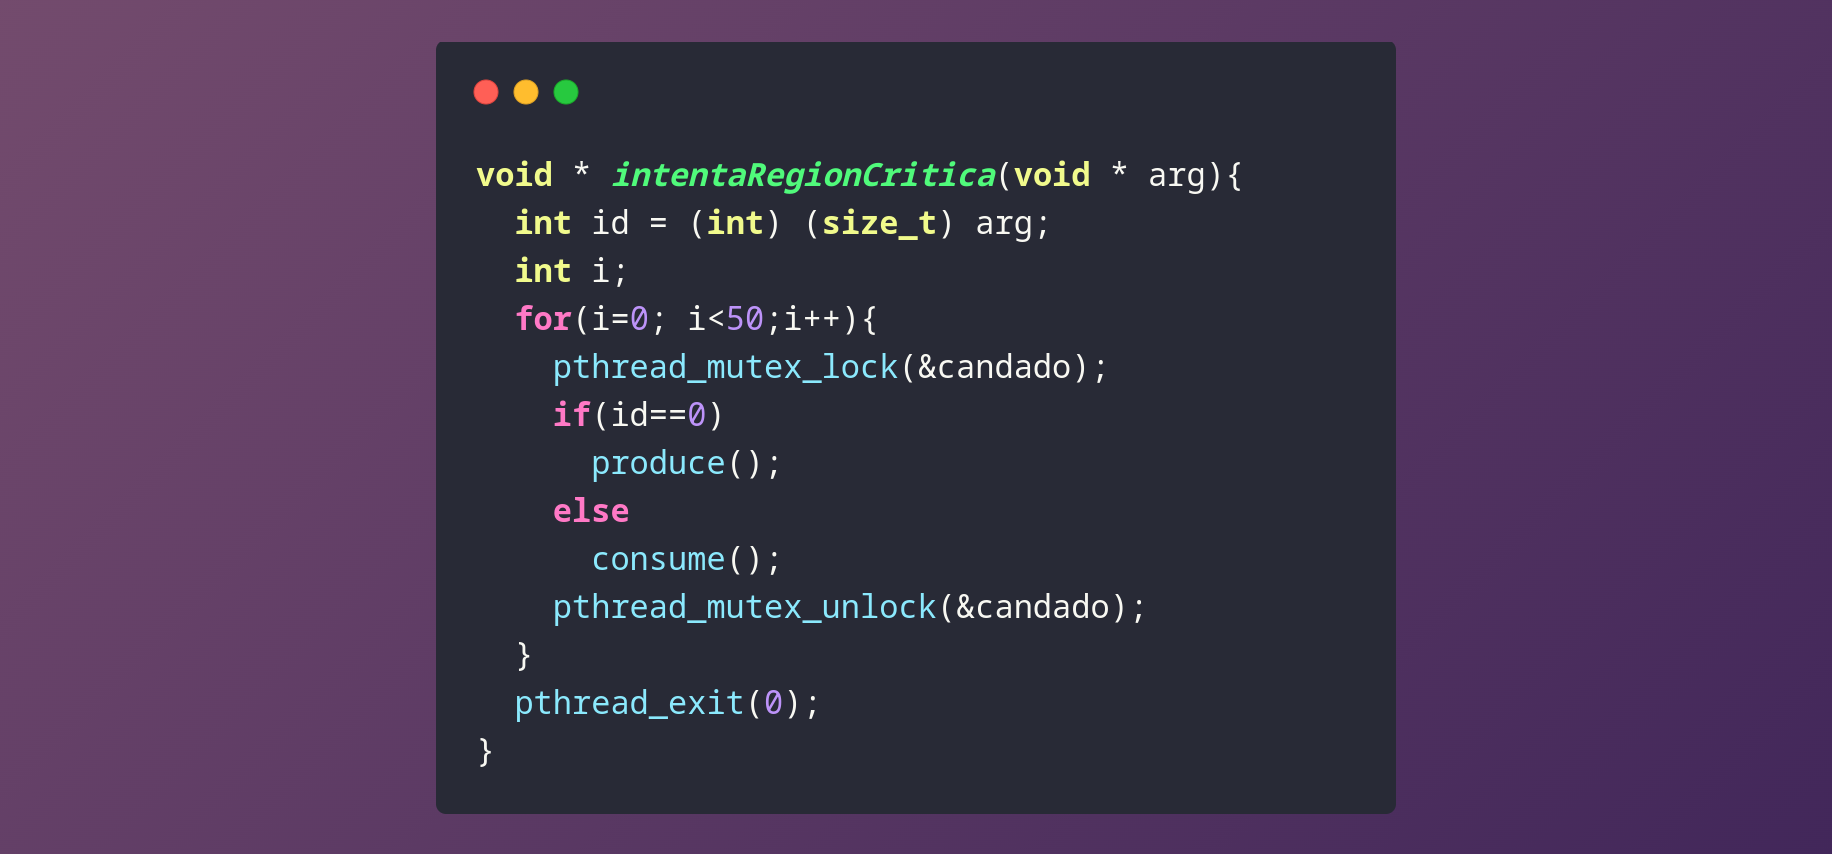
\includegraphics[width=\linewidth]{intentaRC.png}
		\caption{Función intentaRegionCritica}
		\label{fig:intentaRC}
	\end{figure}
	\newpage
	\subsection{Función 'consume'}
	Esta función nos permitirá consumir los productos del almacén para ello utilizamos primero un condicional para el caso donde el la posición del almacén sea igual a cero, esto ocurre porque no tenemos elementos en el almacén, no tiene sentido que consumamos, por lo que se dormirá este proceso. 
	Por otro lado , en cualquier otra posición se debería de consumir  el producto, que en este caso lo hace asignando el carácter nulo y restando uno a posición, para notarlo imprimimos el \emph{almacén} para notar las diferencias. Por ultimo despertamos al otro hilo para que pueda producir. Cabe notar que esta función solamente aplica a los dos primeros códigos, ya que en el tercero necesitaremos otras condicionales, que son muy parecidas. 
	\begin{figure}[h!]
		\centering
		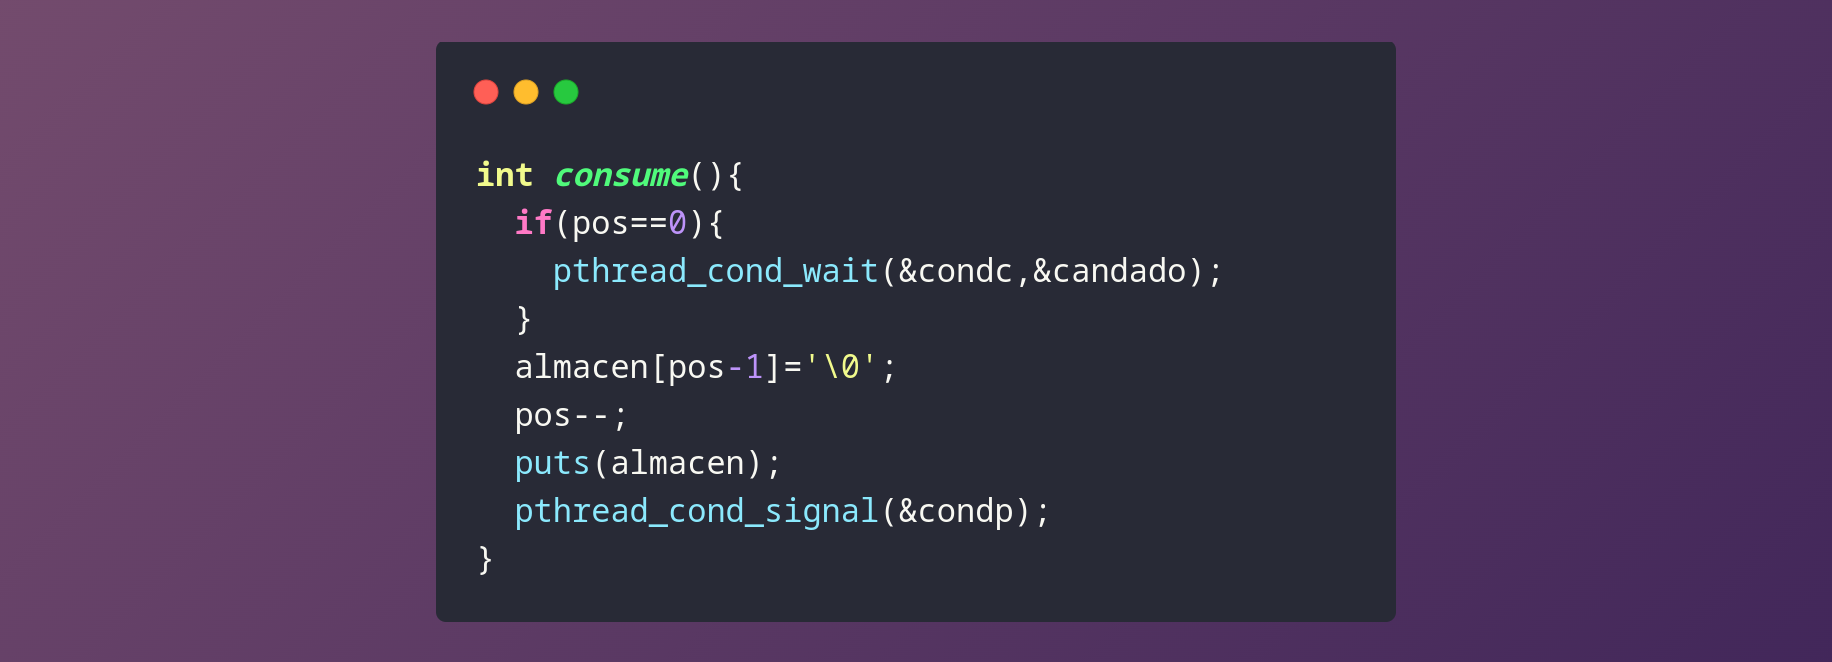
\includegraphics[width=\linewidth]{consume.png}
		\caption{Función 'consume'}
		\label{fig:consume}
	\end{figure}
	\subsection{Función 'produce'}
	Para el caso de producir, tendremos una versión muy parecida para los dos primeros códigos, ya que solamente tendremos que cambiar la posición con la que es comparado; es decir, en el primer código se compara con diez, para dormir a este hilo cuando se ha llenado el almacén y en caso del segundo condigo se compara con uno para que el hilo se duerma cuando tiene un solo elemento en el almacén.
	\\\\
	Por otro lado cuando no ocurra que el hilo no este en esas posiciones del almacén  hará las operaciones que normalmente hace, que es producir en la posición actual y adelantarse una posición, ademas de despertar al otro hilo al final de esto, esto con la finalidad de que los dos compitan de nuevo por tomar la región critica y escribir sobre ella.  
	\begin{figure}[h!]
		\centering
		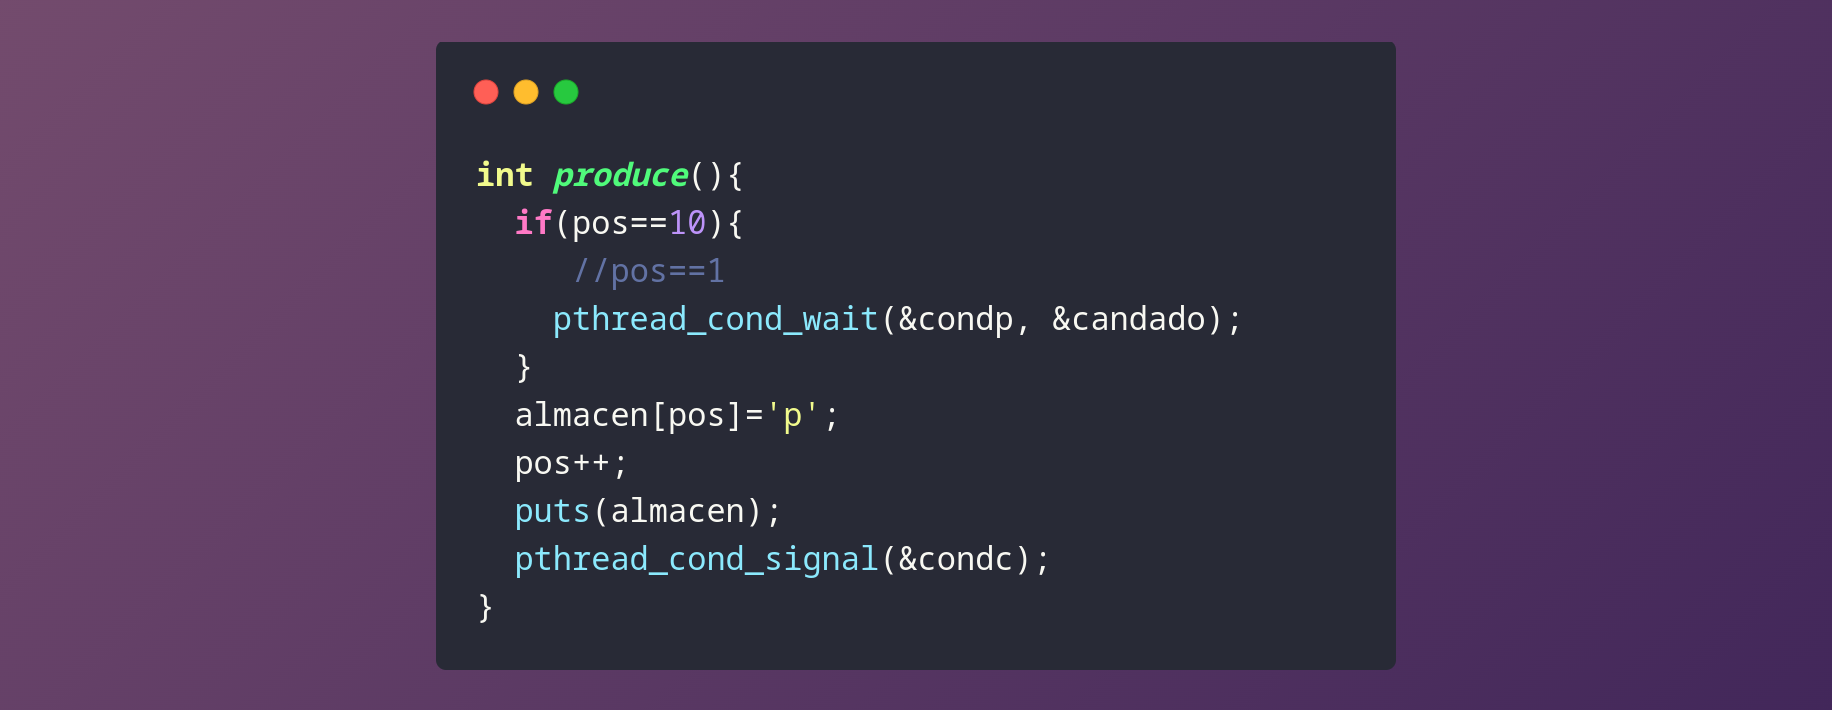
\includegraphics[width=\linewidth]{produce.png}
		\caption{Función 'produce'}
		\label{fig:produce}
	\end{figure}
	\subsection{Función 'consume' para el tercer código}
	Debido a que en el último caso queremos garantizar que se consuman siete productos antes de volver a producir, dado que en la producción se crean siete productos antes de que se comience a consumir; tendremos que hacer un par de cambios para que esto se vea reflejado. 
	\\
	Notaremos que en caso de que la posición sea cero despertará al otro hilo y se dormirá el mismo, en caso de que hayamos realizado un total de noventa y ocho elementos entonces despertamos al otro hilo y salimos del programa, justamente con el fin de que no se interbloqueen los hilos, ya que en esa posición el hilo estaría dormido. En cualquier otro caso realiza la misma tarea que en los códigos pasados, con la excepción de que no despierta al otro hilo. 
	\begin{figure}[h!]
		\centering
		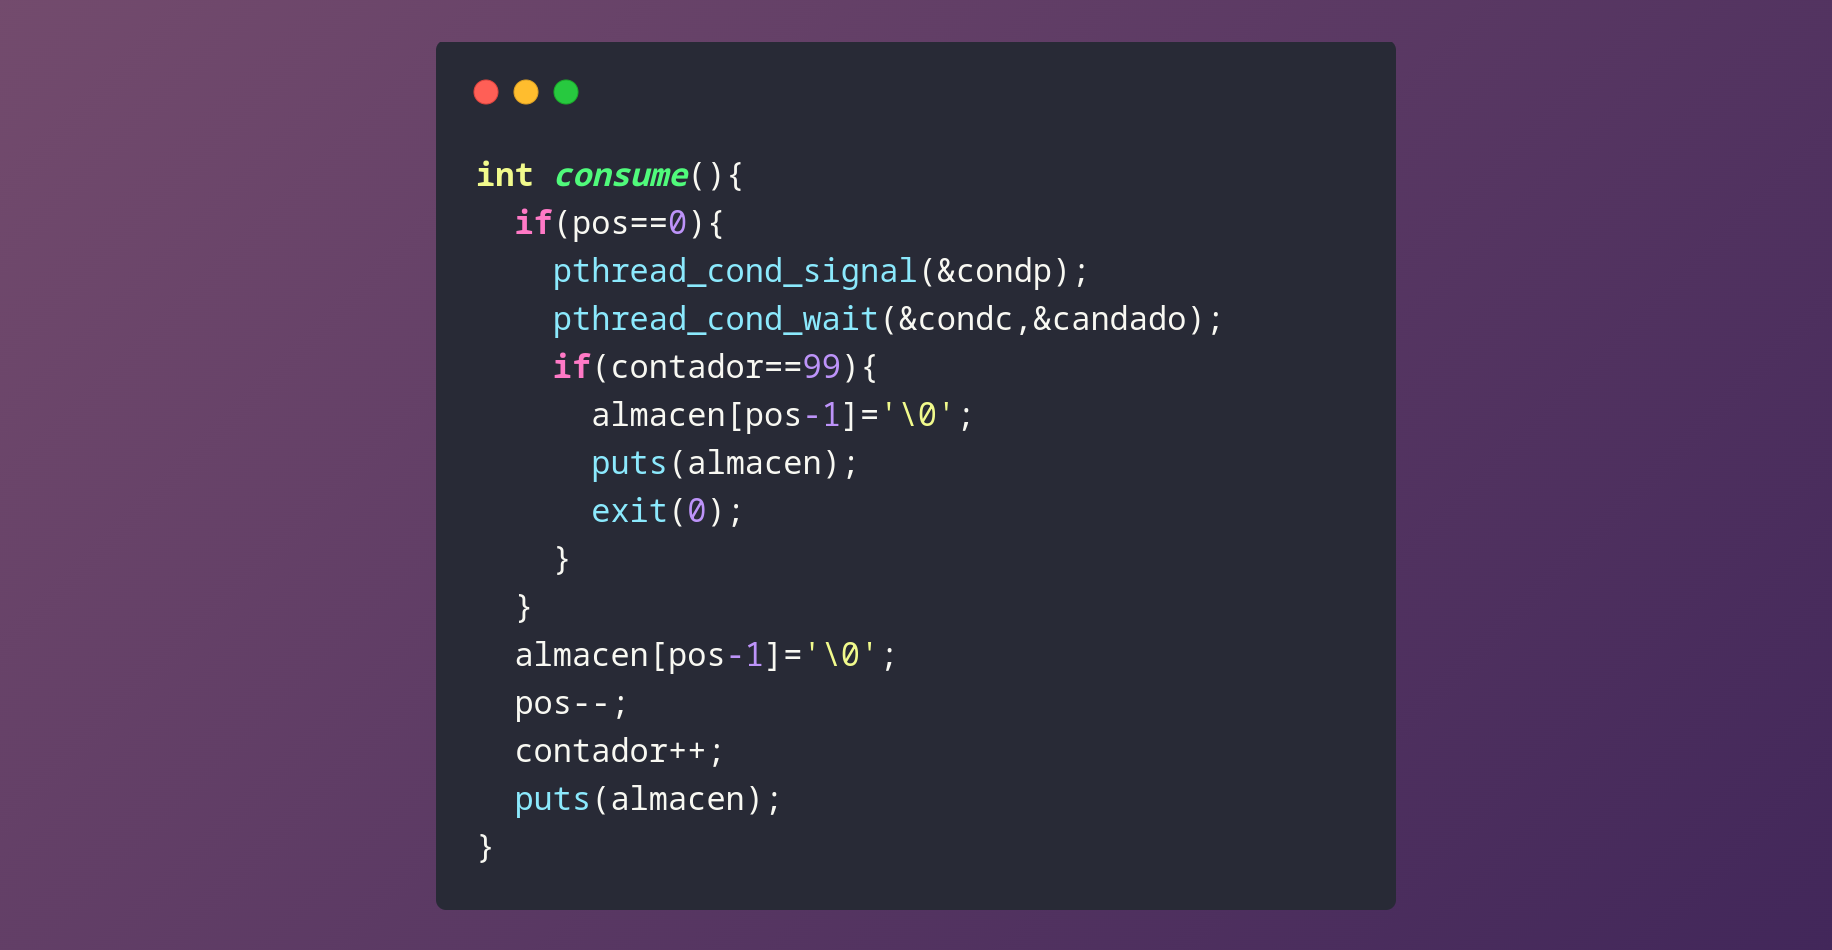
\includegraphics[width=\linewidth]{consumev2.png}
		\caption{Función 'consume'}
		\label{fig:consumev2}
	\end{figure}
	\newpage
	\subsection{Función 'produce' para el tercer código}
	En este caso tenemos la misma situación, cuando la posición sea igual a siete tendremos lo mismo, se despertará al hilo de lo producción y se dormirá el otro hilo, tanto en este como el caso en el que se consume se producirán siete y se consumirán siete obligadamente. Luego, cuando tengamos que el contador llego al ultimo elemento despertamos al otro hilo y terminamos el programa. 
	\\
	En el caso contrario, donde tengamos que ninguna de las dos condiciones se cumplen, entonces tendremos la ejecución "normal" del hilo como en el caso de los otros códigos. 
	\\\\
	Básicamente de esta forma obtenemos los códigos que nos permiten obtener los resultados deseados, cabe aclarar que en el caso del segundo código no es necesario hacer estas últimas condiciones ya que pasa de uno a otro constantemente, dicho de otra forma, solamente alterna entre dos estados y en cada uno de esos estados se despierta al hilo contrario, que era justamente lo que sucedía en el último caso; los dos hilos se podían bloquear y dejar al procesos en un estado de espera perpetuo. 
	\begin{figure}[h!]
	\centering
	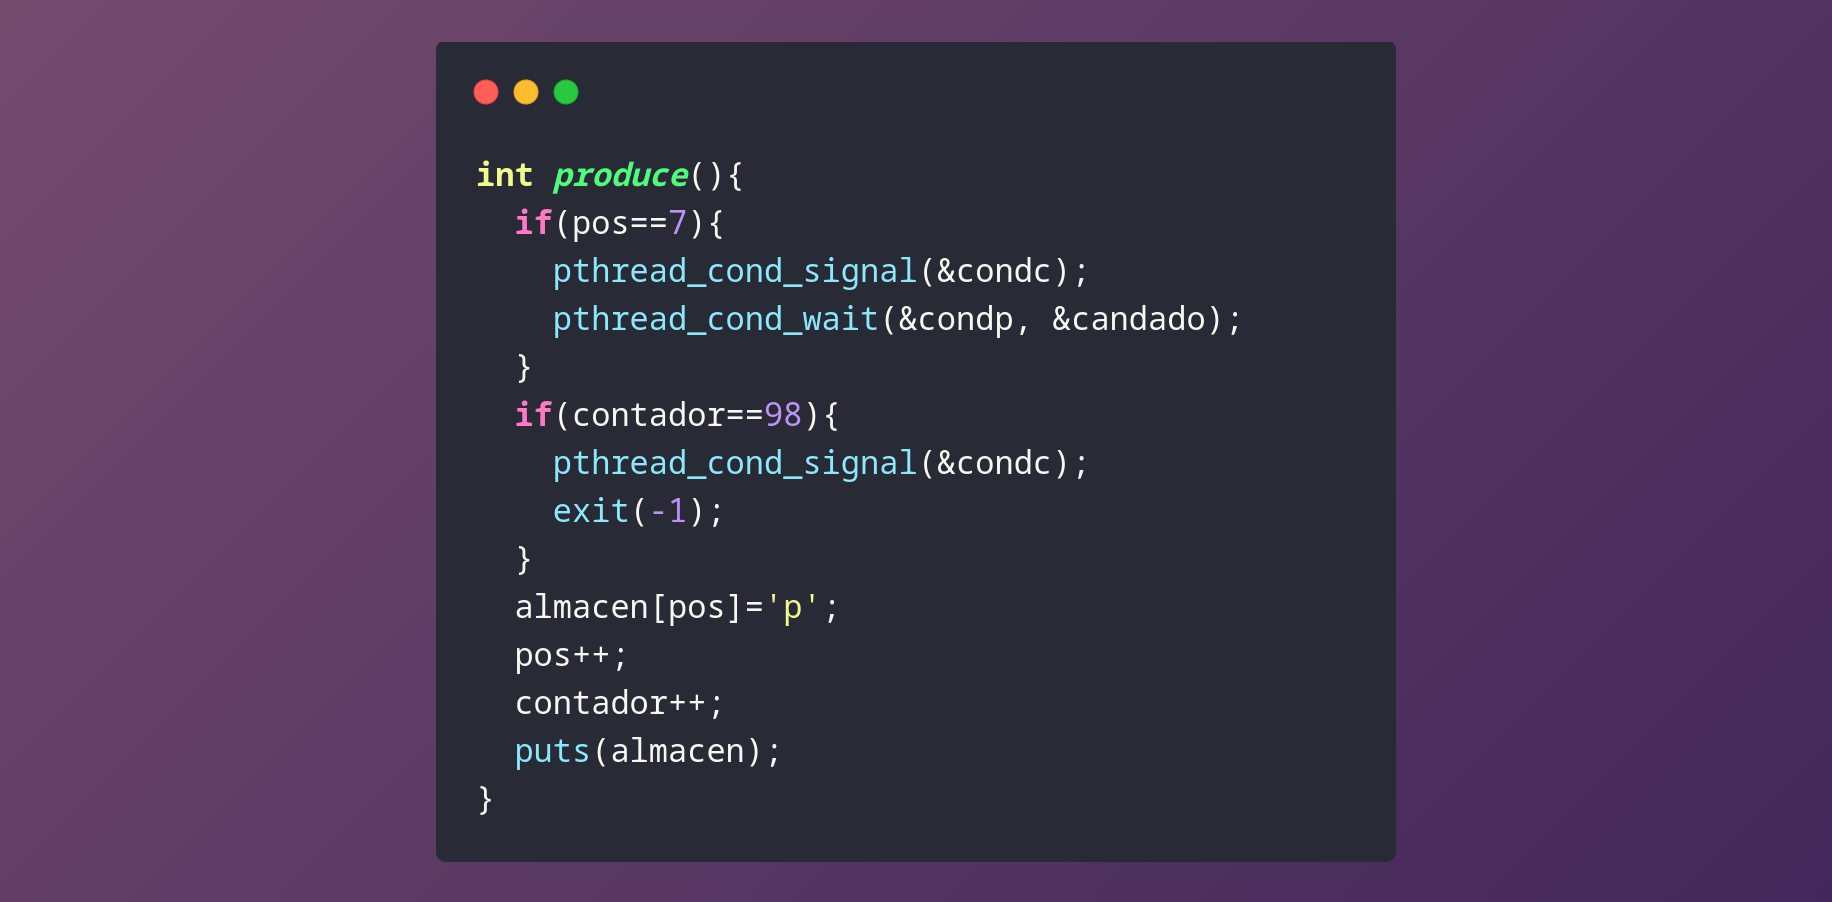
\includegraphics[width=\linewidth]{producev2.png}
	\caption{Función 'produce'}
	\label{fig:producev2}
	\end{figure}
	\newpage
	\section{Resultados}
	\begin{figure}[h!]
		\centering
		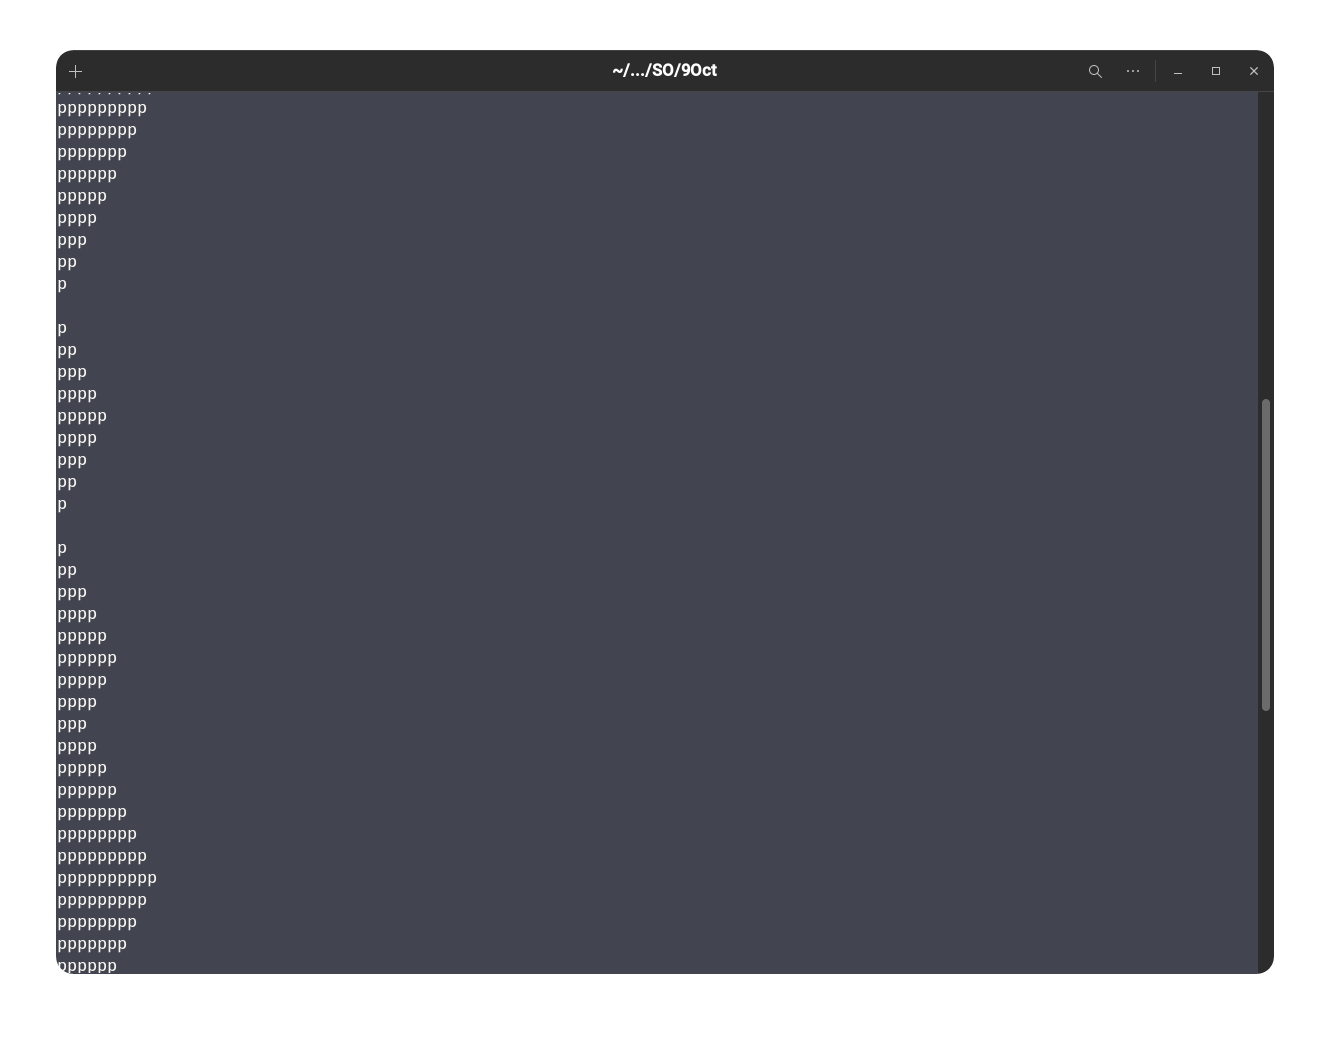
\includegraphics[width=0.7\linewidth]{res1}
		\caption{Resultados primer código}
		\label{fig:res1}
	\end{figure}
	\begin{figure}[h!]
		\centering
		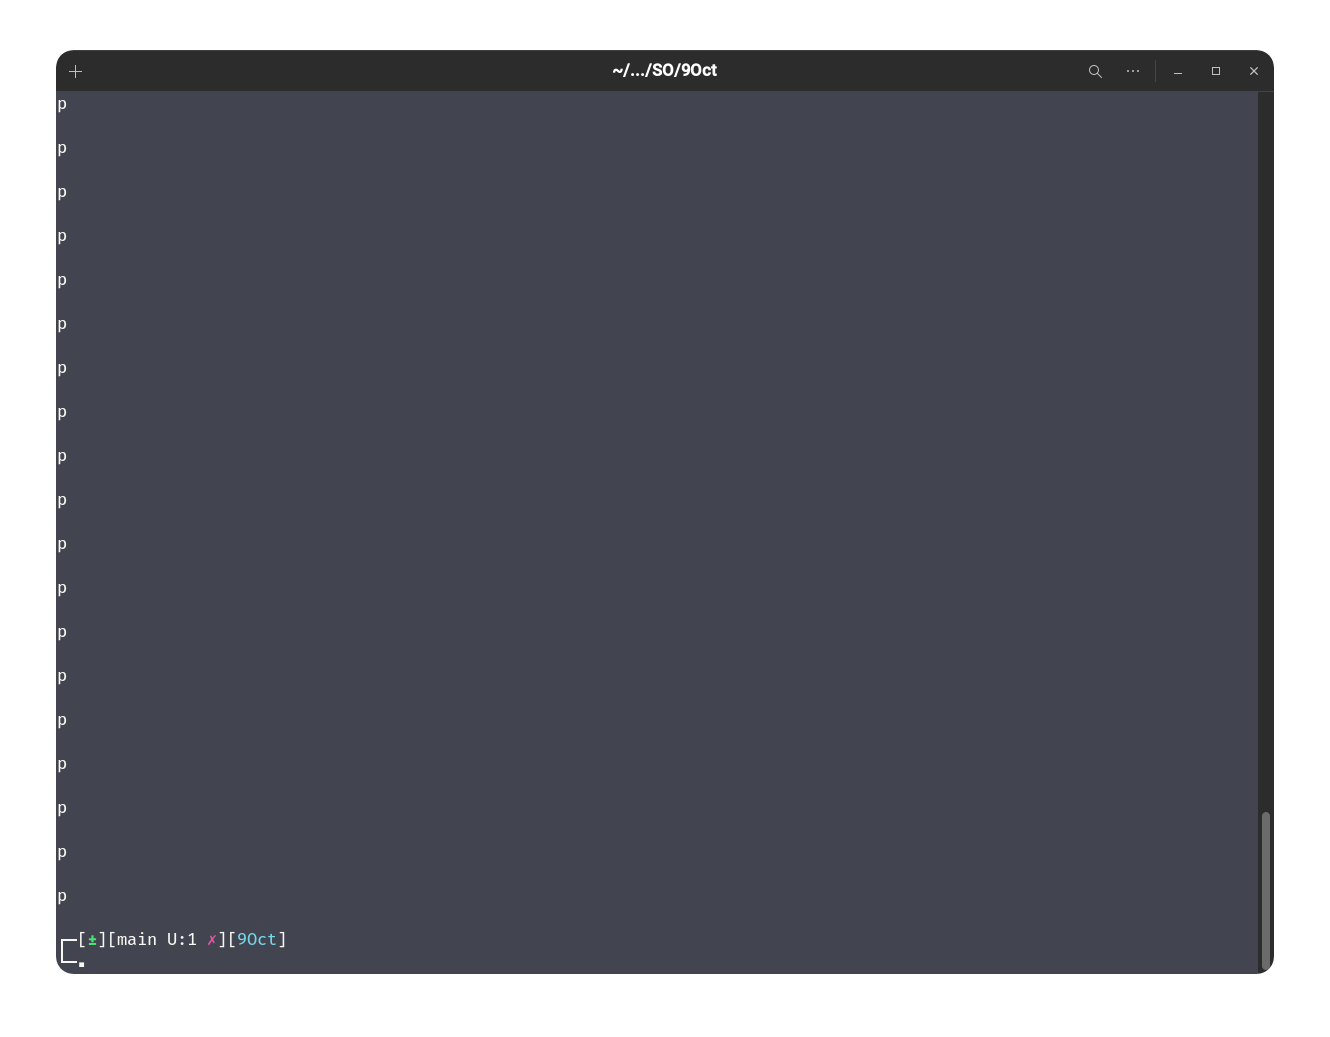
\includegraphics[width=0.7\linewidth]{res2}
		\caption{Resultado segundo código}
		\label{fig:res2}
	\end{figure}
	\begin{figure}[h!]
		\centering
		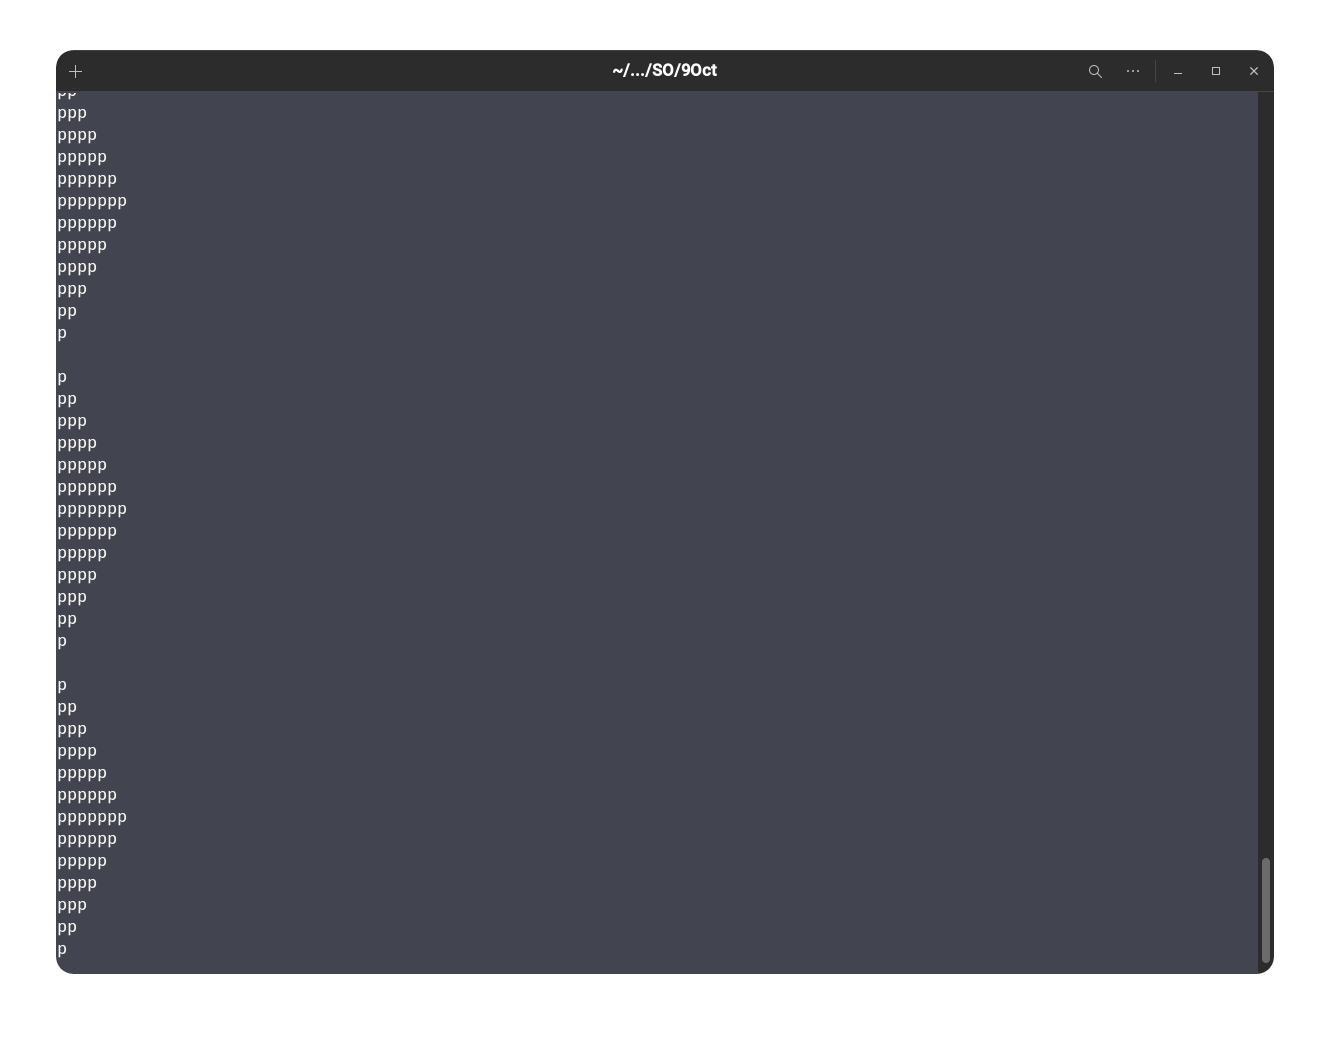
\includegraphics[width=0.7\linewidth]{res3}
		\caption{Resultado tercer código}
		\label{fig:res3}
	\end{figure}
	\newpage
	\section{Preguntas}
	\begin{enumerate}
		\item ¿Qué son las condiciones de carrera?
		\\Es como una especie de competencia entre diferentes cosas para lograr un objetivo, básicamente son dos procesos o hilos peleando por obtener algo en particular, en este caso un recurso para hacer uso de el. 
		\item  ¿Qué es la exclusión mutua?
		\\ Es la solución a las condiciones de carrera, garantiza que el acceso a un recurso compartido se hace de manera ordenada y uno a la vez, osea que no tenemos sobre escrituras de los recursos o cosas por el estilo.  
		\item ¿Qué pasa si tanto el productor como el consumidor despiertan a su contraparte una vez que han salido de su región crítica?¿Cuál es la diferencia con respecto a no hacerlo?
		\\ Puede que al despertarlos tengamos un problema de sobreescrirura justamente, porque todo lo que no esta dentro de la región critica es probable que sea modificado, de igual manera podría ocurrir que haya un interbloqueo de los procesos por las condiciones de carrera en busca del recurso. Si no lo hacemos es claro que el programa no tendrá problema alguno dentro de sus región critica aseguramos el uso correcto y ordenado de los recursos compartidos. Además no garantizaría la exclusión mutua. 
		\item ¿En qué momento se generan condiciones de carrera en su programa? Indique la sección.
		\\En todos los códigos se genera una condición de carrera en el momento que decidimos escribir en el arreglo denominado como \emph{almacén}, en ese punto los procesos se pelean por el recurso, de hecho después de que se despiertan uno a otros vuelve a ocurrir, solamente que ahora es de manera ordenada.
		\item Indique las regiones críticas en su código e inclúyalas en su reporte. Justifique su respuesta
		\begin{figure}[h!]
			\centering
			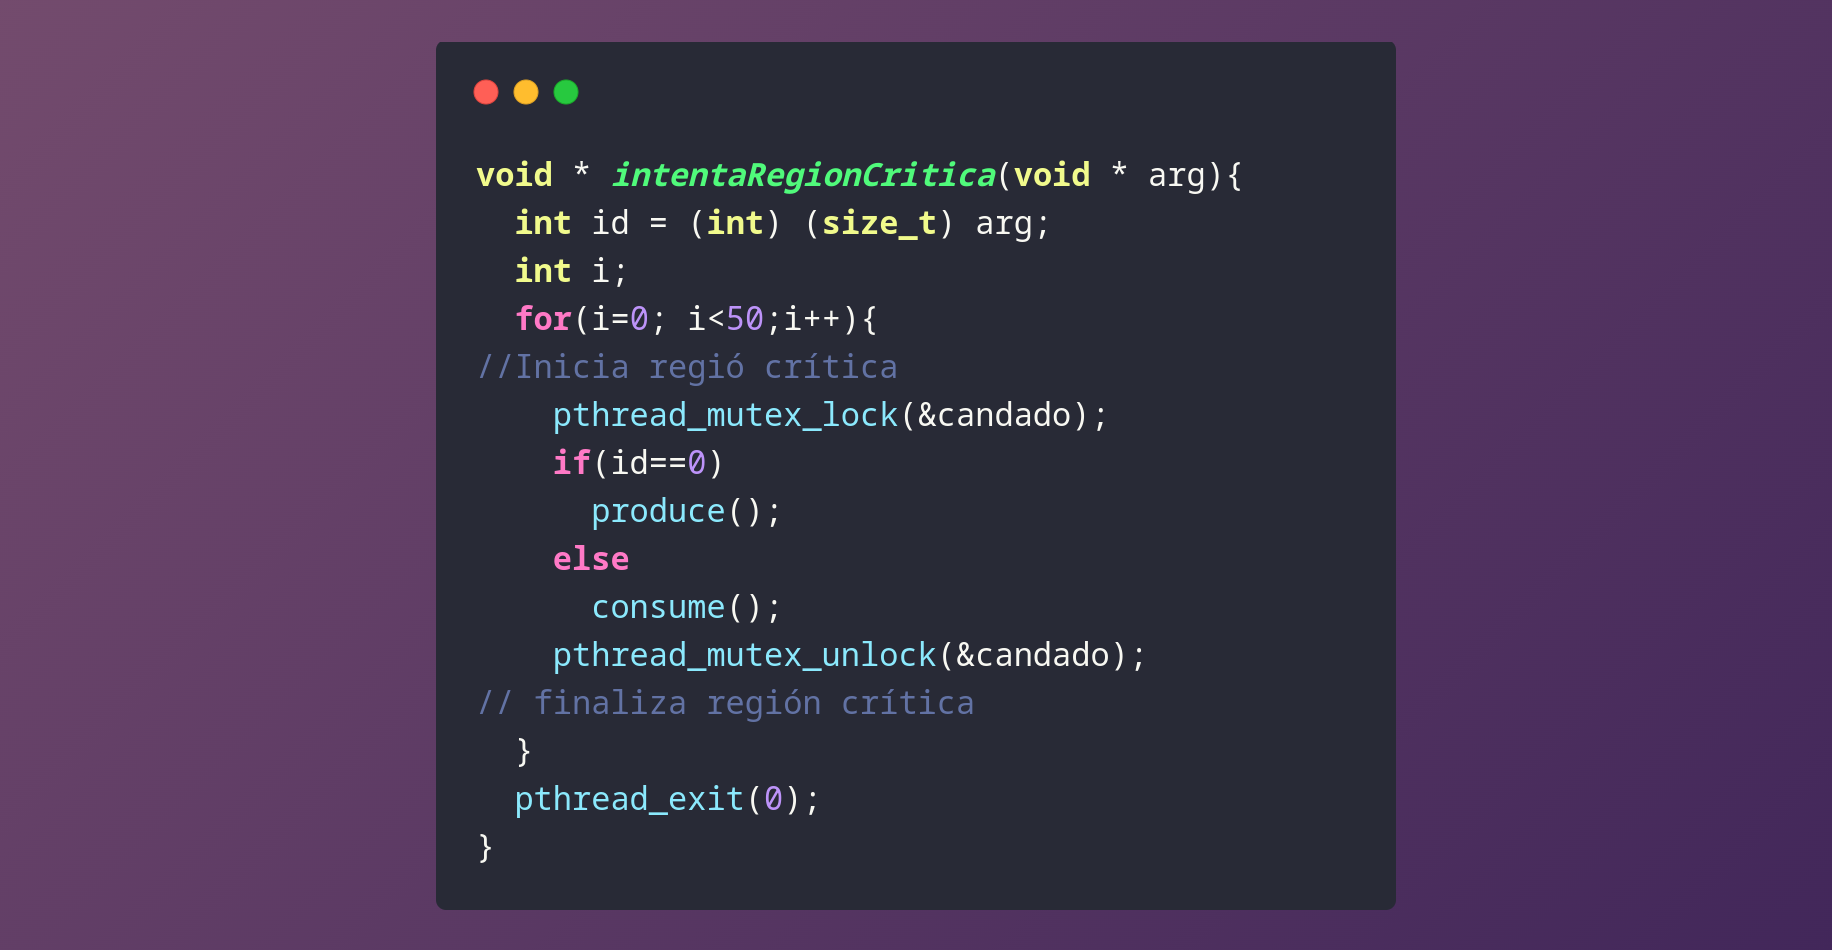
\includegraphics[width=0.9\linewidth]{p1}
			\caption{Regiones Críticas}
			\label{fig:p1}
		\end{figure}
		\item ¿Qué solución implementó para garantizar exclusión mutua?
		 \\En este caso se utilizó Mutex para que justamente bloqueemos el acceso a la región critica, además se hizo uso de condicionales para despertar o dormir hilos, todo ello con el afán de que tengamos mejo manejo de los datos en la región critica, dado que necesitamos de ciertas condiciones. 
		\end{enumerate}
	
\end{document}